%\FloatBarrier
\subsection{Neo Burst Performance Characteristics}
Previous experiments \citep{dahlgren2013} had the operator sitting up all night waiting for aurora to press Record.
This level of human effort is not sustainable in the long term.
Obviously this method misses the build up time to interesting events, and stands a good chance of missing the desired events as well.
Nonetheless, this is how much high-speed auroral observation has taken place prior to about 2010.

For \citet{dahlgren2013} to achieve usable frame rates at full resolution, burst mode was used.
Burst mode uses the on-board camera memory in a short burst, upon which recording stops and the camera RAM is read to the PC RAM over the 3-tap Cameralink interface.
Neither binning or reducing width (width is the 2560 pixel dimension) helps improve frame rates.
Measurements were taken in Table~\ref{tab:neofullburst} at full frame.
\unit[$10^{-5}$]{s} is the minimum possible exposure time of Neo, which is much too short for auroral observations.
\unit[$10^{-3}$]{s} is roughly the minimum useful exposure time for aurora.
\unit[$10^{-2}$]{s} is about the fastest rate the companion iXon would run at. 
At full frame, the iXon can image at \unit[33]{ms} rate.
\begin{table}\centering
	\caption{Andor Neo full-frame burst imaging characteristics}\label{tab:neofullburst}
	\begin{tabular}{p{5em}p{4.5em}p{4.5em}p{5.5em}p{5em}p{5em}}
		\toprule
		Exp. Time (sec.) &  Width (pixels) & Height (pixels) &  Frames / sec &  Max \# of frames &  Max. Burst Time (sec.) \\
		\midrule
		$10^{-5}$ & 2560 & 2160 & 48.95 & 160 & 3.27 \\
		$10^{-3}$ & 2560 & 2160 & 46.68 & 160 & 3.43 \\
		$10^{-2}$ & 2560 & 2160 & 32.87 & 160 & 4.87 \\
		\bottomrule
	\end{tabular}
\end{table}
To optimize viewing area versus frame rate, the data in Table~\ref{tab:neooptburst} was collected.
Neo burst mode performance is optimized by exploiting Neo sCMOS sensor read geometry (center outward)--center on sensor.
\begin{table}\centering
	\caption{Neo burst performance with less than full-height image}\label{tab:neooptburst}
	\begin{tabular}{p{5em}p{4.5em}p{4.5em}p{5.5em}p{5em}p{5em}}
		\toprule
		Exp. Time (sec.) & Width (pixels) & Height (pixels) & Frames / sec & Max \# of frames & Max. Burst Time (sec.) \\
		\midrule
		$10^{-5}$ & 2560 & 1000 & 103.79 & 344 & 3.31\\
		$10^{-5}$ & 2560 & 512 & 197.58 & 667 & 3.38\\
		$10^{-5}$ & 2560 & 256 & 375.64 & 1315 & 3.5\\
		\midrule
		$10^{-3}$ & 2560 & 1000 & 94.12 & 344 & 3.65\\
		$10^{-3}$ & 2560 & 512 & 165.26 & 667 & 4.04\\
		$10^{-3}$ & 2560 & 256 & 273.82 & 1315 & 4.8\\
		\midrule
		$10^{-2}$ & 2560 & 1000 & 67.53 & 344 & 5.09\\
		$10^{-2}$ & 2560 & 512 & 79.87 & 667 & 8.35\\
		$10^{-2}$ & 2560 & 256 & 88.33 & 1315 & $\rightarrow\infty$\\
		\bottomrule
	\end{tabular}
\end{table}
From Table~\ref{tab:neooptburst} and the lens chosen, useful video is not obtained outside of \unit[5]{s} bursts. 
A sustainable mode of operation preserving FOV but sacrificing the excess resolution was required for the DMC mission.

%\FloatBarrier
\subsection{Neo Sustained Recording Performance Characteristics}
The Andor Neo sustained data rates are \textit{substantially} lower than burst mode rates due to the limited 3-tap Cameralink bandwidth.
The Andor Zyla 10-tap Cameralink has significantly higher frame rates than Neo with same sCMOS sensor.
Binning (creating macropixels by grouping adjacent pixels) is the key to sustained useful recording with the Andor Neo.
The maximum sustained frame rate with the Andor Neo using Solis 4.29.30012.0 is given in Table~\ref{tab:neomax}.
The Neo frame rates at 4x4 and 8x8 binning are comparable with the Andor iXon full frame rate.
\begin{table}\centering
	\caption{Neo maximum sustained frame rate with binning}\label{tab:neomax}
	\begin{tabular}{ccc}
		\toprule
		binning & width x height & frames / sec \\
		\midrule
		1x1 & 2560 x 2160 & 20 \\
		2x2 & 1280 x 1080 & 32 \\
		4x4 & 640 x 540 & 54 \\
		8x8 & 320 x 270 & 109 \\
		\bottomrule
	\end{tabular}
\end{table}


%\FloatBarrier
\subsection{Andor Neo DMC Resolution}
The Andor Neo camera has excess resolution for the planned FOV, so the Neo was typically binned 8x8.
An example of the excellent resolution of a splitting auroral arc at these Neo settings is given in Figure~\ref{fig:neosplit}.
\begin{figure}
	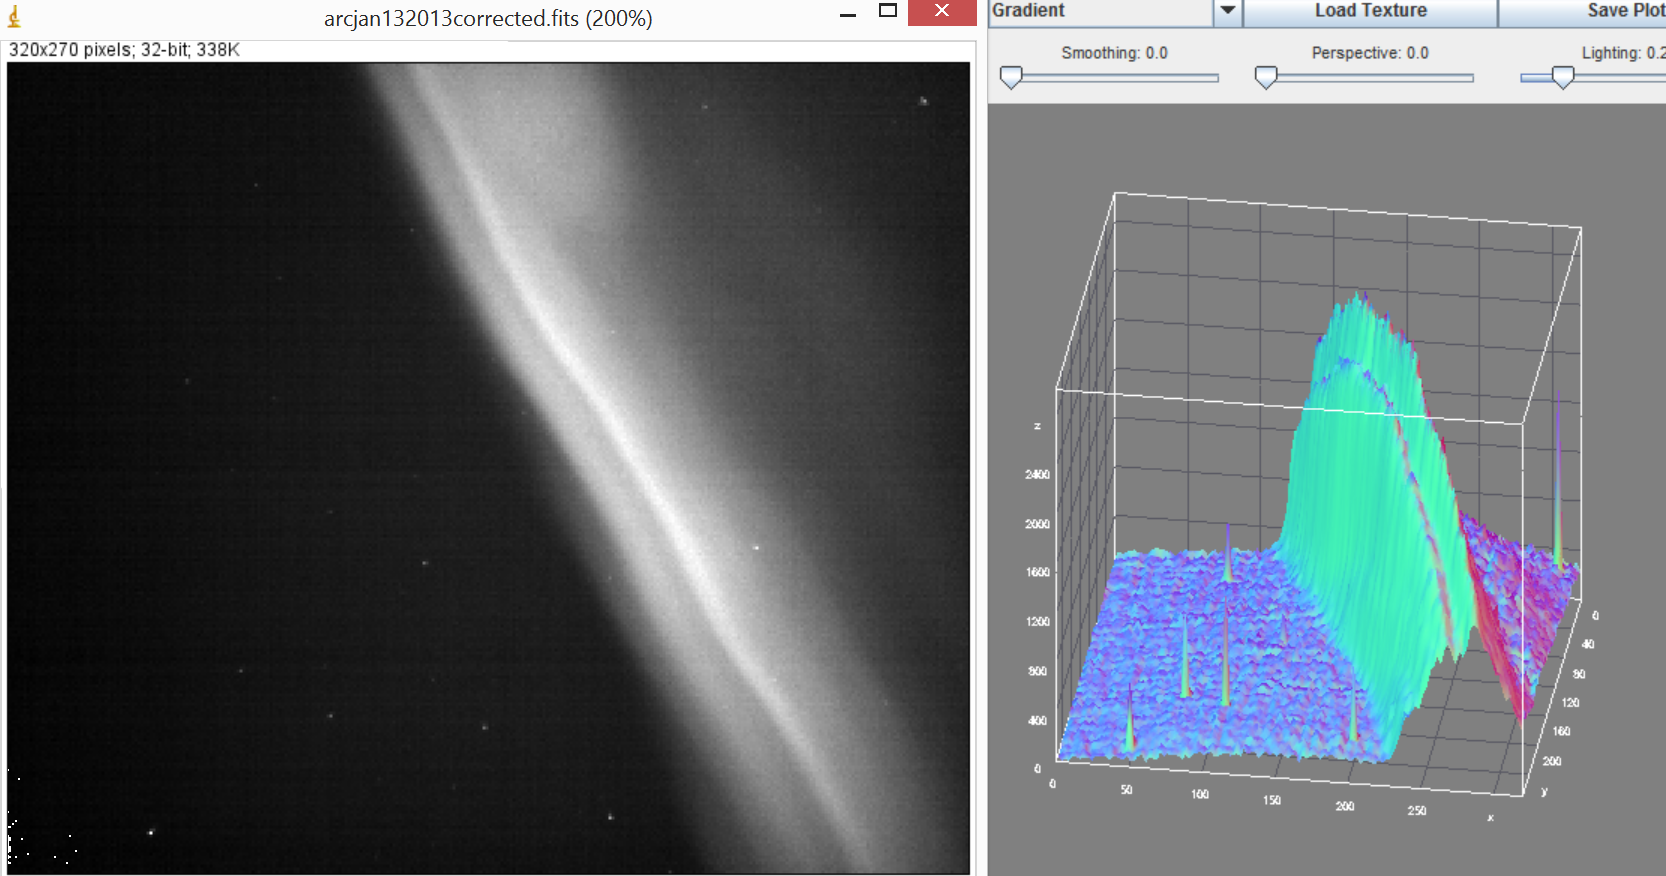
\includegraphics[trim=0 0 50 40,clip,width=\linewidth]{gfx/2013-01-13gradient}
	\caption{Splitting arc seen by DMC Neo camera, Jan 13, 2013}\label{fig:neosplit}
\end{figure}
The 3-D view of image intensity seen in the right panel of Figure~\ref{fig:neosplit} shows the fine quality of the focus and resolution with stars appearing as isolated peaks that stay nearly constant from one frame to the next.
